\PassOptionsToPackage{usenames,dvipsnames}{xcolor}

\documentclass[20pt, a0paper, landscape, margin=0mm, innermargin=15mm, blockverticalspace=15mm, colspace=15mm, subcolspace=8mm]{tikzposter}
\usepackage[T1]{fontenc}
\usepackage[utf8]{inputenc}
\usepackage[english]{babel}

\usepackage{amsmath,amsfonts,amssymb,mathtools}

%\usepackage[usenames,dvipsnames]{xcolor}
\usepackage{graphicx,mwe}
\usepackage{filecontents}% http://ctan.org/pkg/filecontents
\usepackage{tikz}
\usepackage{multicol}
\usepackage{adjustbox}
\usepackage{authblk}

\usepackage{enumitem}

\usepackage{caption}
\captionsetup{font=large}

\usepackage{url}
\usepackage[colorlinks=false]{hyperref}
\urlstyle{tt}


%\newcommand*{\doi}[1]{\href{https://doi.org/#1}{\nolinkurl{https://doi.org/#1}}}
\newcommand*{\doi}[1]{\href{https://doi.org/#1}{\nolinkurl{doi:#1}}}


% university colors based on branding guides
\definecolor{OSUorange}{HTML}{C34500}
\definecolor{UConnBlue}{HTML}{000E2F}
\definecolor{GoogleBlue}{HTML}{0266C8}

% \makeatletter
% \def\TP@titlegraphictotitledistance{-4cm}
% \settitle{ \centering \vbox{
% \@titlegraphic \\ [\TP@titlegraphictotitledistance]
% \centering
% \color{titlefgcolor} {\bfseries \Huge \@title \par} % add \sc for smallcaps
% \vspace*{2em}
% {\huge \@author \par} \vspace*{1em} {\LARGE \@institute}
% }}
% \makeatother

%% Code for increasing tikzfigure caption font size
% \renewenvironment{tikzfigure}[1][]{
%   \def \rememberparameter{#1}
%   \vspace{10pt}
%   \refstepcounter{figurecounter}
%   \centering
%   }{
%     \ifx\rememberparameter\@empty
%     \else %nothing
%     \\[10pt]
%     {\large Fig.~\thefigurecounter: \rememberparameter}
%     \fi
% }


%% Set up a logo on each side
\makeatletter
\newcommand\insertlogoi[2][]{\def\@insertlogoi{\includegraphics[#1]{#2}}}
\newcommand\insertlogoii[2][]{\def\@insertlogoii{\includegraphics[#1]{#2}}}
\newlength\LogoSep
\setlength\LogoSep{-2cm}

%\insertlogoi[width=18cm]{logo-CMYK-horizontal}
%\insertlogoii[width=18cm]{OSU-color-horz}

\def\TP@titlegraphictotitledistance{-4cm}
\settitle{ \centering \vbox{
%\@titlegraphic \\ [\TP@titlegraphictotitledistance]
\centering
\color{titlefgcolor} {\bfseries \Huge \@title \par} % add \sc for smallcaps
\vspace*{2em}
{\huge \@author \par} \vspace*{1em} {\LARGE \@institute}
}}

\renewcommand\maketitle[1][]{  % #1 keys
    \normalsize
    \setkeys{title}{#1}
    % Title dummy to get title height
    \node[transparent,inner sep=\TP@titleinnersep, line width=\TP@titlelinewidth, anchor=north, minimum width=\TP@visibletextwidth-2\TP@titleinnersep]
        (TP@title) at ($(0, 0.5\textheight-\TP@titletotopverticalspace)$) {\parbox{\TP@titlewidth-2\TP@titleinnersep}{\TP@maketitle}};
    \draw let \p1 = ($(TP@title.north)-(TP@title.south)$) in node {
        \setlength{\TP@titleheight}{\y1}
        \setlength{\titleheight}{\y1}
        \global\TP@titleheight=\TP@titleheight
        \global\titleheight=\titleheight
    };

    % Compute title position
    \setlength{\titleposleft}{-0.5\titlewidth}
    \setlength{\titleposright}{\titleposleft+\titlewidth}
    \setlength{\titlepostop}{0.5\textheight-\TP@titletotopverticalspace}
    \setlength{\titleposbottom}{\titlepostop-\titleheight}

    % Title style (background)
    \TP@titlestyle

    % Title node
    \node[inner sep=\TP@titleinnersep, line width=\TP@titlelinewidth, anchor=north, minimum width=\TP@visibletextwidth-2\TP@titleinnersep]
        at (0,0.5\textheight-\TP@titletotopverticalspace)
        (title)
        {\parbox{\TP@titlewidth-2\TP@titleinnersep}{\TP@maketitle}};

    % \node[inner sep=0pt,anchor=west]
    %   at ([xshift=-\LogoSep]title.west)
    %   {\@insertlogoi};
    %
    % \node[inner sep=0pt,anchor=east]
    %   at ([xshift=\LogoSep]title.east)
    %   {\@insertlogoii};

    % Settings for blocks
    \normalsize
    \setlength{\TP@blocktop}{\titleposbottom-\TP@titletoblockverticalspace}
}
\makeatother

\setlength{\columnsep}{2cm}


\title{\parbox{0.7\linewidth}{\centering Software citation principles for credit and reuse}}

\author[1]{Kyle E.\ Niemeyer}
\author[2]{Daniel S.\ Katz}
\author[3]{Arfon M.\ Smith}

\affil[1]{School of Mechanical, Industrial, and Manufacturing Engineering, Oregon State University}
\affil[2]{National Center for Supercomputing Applications \& Electrical and Computer Engineering
Department \& \authorcr School of Information Sciences, University of Illinois at Urbana--Champaign}
\affil[3]{Data Science Mission Office, Space Telescope Science Institute}

\institute{
\href{mailto:kyle.niemeyer@oregonstate.edu}{\nolinkurl{kyle.niemeyer@oregonstate.edu}} and
\href{mailto:dskatz@illinois.edu}{\nolinkurl{dskatz@illinois.edu}} and
\href{mailto:arfon@stsci.edu}{\nolinkurl{arfon@stsci.edu}}
}

\date{}



\usetitlestyle{Filled}

\begin{document}

\maketitle

\begin{columns} % See Section 4.4

    \column{0.7}
    \block{Software Citation Principles}{

    \begin{tikzfigure}
    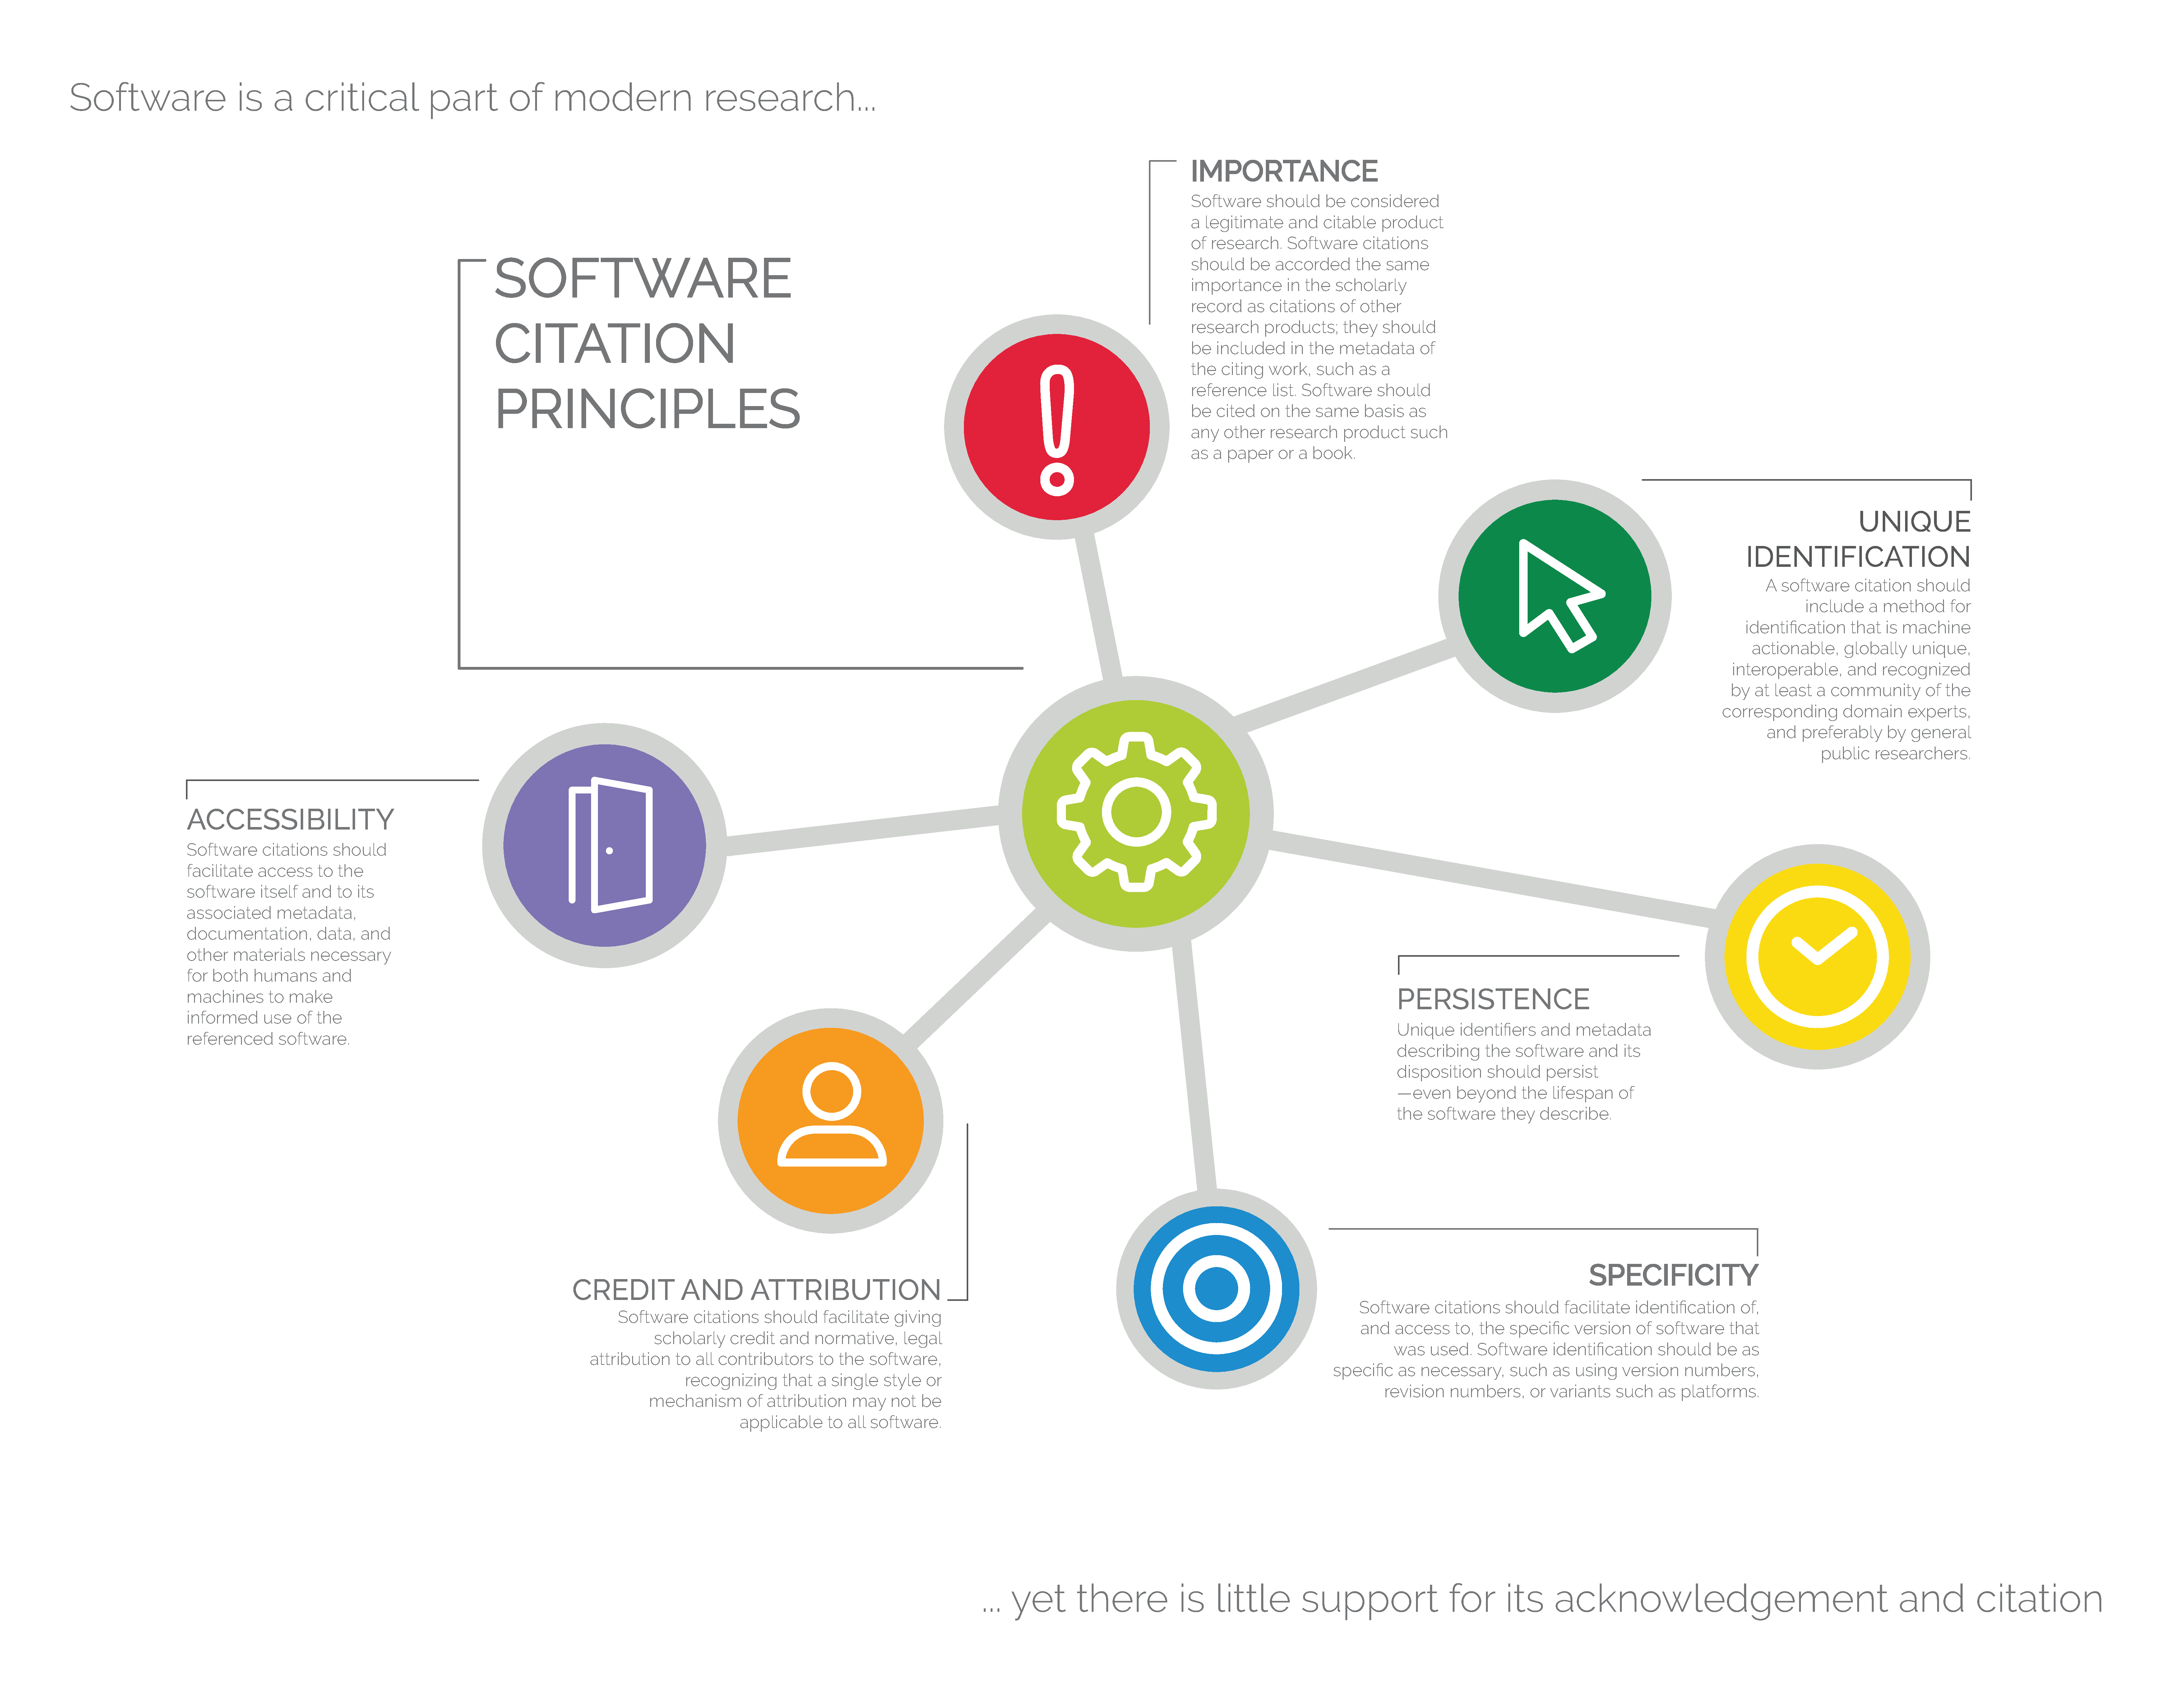
\includegraphics[width=0.95\linewidth]{full-white}
    \end{tikzfigure}
    %
    }

    \column{0.3}
    \block{Organizations}{

    \begin{tikzfigure}
    
\includegraphics[width=0.85\linewidth]{logo-CMYK-horizontal}
    \end{tikzfigure}
    \captionof*{figure}{\url{https://www.force11.org/group/software-citation-working-group}}

    %\vspace{1em}

    \begin{tikzfigure}
    
\includegraphics[width=0.7\linewidth]{OSU-color-horz}
    \end{tikzfigure}
    \begin{tikzfigure}
    
\includegraphics[width=0.75\linewidth]{uclogo_horz_bold}
    \end{tikzfigure}
    \begin{tikzfigure}
    
\includegraphics[width=0.75\linewidth]{stsci_pri_combo_mark_horizonal_white_bkgd}
    \end{tikzfigure}
    }

    \block{Further Information}{
    %
    \begin{enumerate}[leftmargin=1cm,topsep=0pt]

        \item AM Smith, DS Katz, KE Niemeyer, \& FORCE11 Software Citation Working Group.
        ``Software citation principles.'' (2016) \textit{PeerJ Computer Science}, 2:e86.
        \doi{10.7717/peerj-cs.86}

        \item KE Niemeyer, AM Smith, \& DS Katz.
        ``The challenge and promise of software citation for credit, identification, discovery, and reuse.'' (2016) \textit{ACM Journal of Data and Information Quality}, 7(4):16.
        \doi{10.1145/2968452}

        \item DS Katz, KE Niemeyer, \& AM Smith.
        ``Strategies for biomedical software management, sharing, and citation.'' (2016) \textit{PeerJ Preprints} 4:e2640v1.
        \doi{10.7287/peerj.preprints.2640v1}

        \item DS Katz, KE Niemeyer, AM Smith, WL Anderson, C Boettiger, K Hinsen, R Hooft, M Hucka, A Lee, F L\"{o}ffler, T Pollard, \& F Rios.
        ``Software vs.\ data in the context of citation.'' (2016) \textit{PeerJ Preprints} 4:e2630v1.
        \doi{10.7287/peerj.preprints.2630v1}

        \end{enumerate}

        \begin{minipage}{0.42\linewidth}
            \begin{tikzfigure}
                
\includegraphics[width=\linewidth]{cc-by}
            \end{tikzfigure}
        \end{minipage}
        \hfill
        \begin{minipage}{0.55\linewidth}
        This work is licensed under a Creative Commons Attribution 4.0 International License. To view a copy of this license, visit \url{http://creativecommons.org/licenses/by/4.0/}.
        \end{minipage}
    %
    }
\end{columns}

\end{document}
